\paragraph{Datasets} 
EPIC-KITCHENS is the largest egocentric dataset. Compared to other egocentric datasets such as GTEA \cite{5995444} and cooking datasets such as 50Salads \cite{10.1145/2493432.2493482} and Breakfast \cite{6909500}, EPIC-KITCHENS contains much longer videos and richer verb classes. In addition, while 50Salads  mostly contains consecutive actions, actions in EPIC-KITCHENS are usually separated by background frames where no action is being performed. These background frames comprise a significant portion of all frames (about 32\%) and affect the performace of baseline models, especially the simpler ones. 

\paragraph{FC}
A 2-layer fully connected network is trained with batch size 16 for 50 epochs. The input frames are down-sampled to 1.25FPS. Since the classification is performed frame-wise and considers no temporal relations, the result is highly fragmental. We further note that the model tends to overfit at an early stage. The poor generalizability is indicated by the relatively low Edit score and Figure \ref{fig:baseline_qualitative}. %TODO: include graph. 

% $26.5\%$ of them were background and $13.5\%$ of them were the wash verb class. %
\paragraph{MSTCN} MSTCN demonstrates its effectiveness in segmenting out the most frequent label classes. The top 5 most frequent labels in the training set in EPIC-KITCHENS are the background, \emph{wash}, \emph{take}, \emph{put}, and \emph{cut} class. We observe that the model assigns one of the most frequent verb classes when it struggles to label the action classes. The result implies that the model is able to memorize the label frequency. One potential way to alleviate this situation is to normalize the frequency through the positional weights supplied to each class label.

EPIC-KITCHENS is more complex than the benchmark datasets in many aspects, such as longer video durations and thus more actions involved. We accounted for this increase in complexity by using 15-layer single-stage TCNs rather than the 10-layer ones which are claimed to achieve optimal performance in the original experiment \cite{8953830}. Our experiment shows that there is an improvement in when using a more complex model.

\paragraph{DTGRM} The DTGRM model builds off MSTCN by adding an additional fine-tuning component that refines segmentation around the boundaries. Similar to MSTCN, DTGRM is able to output reasonable segmentation results. \ref{fig:baseline_qualitative} shows that one of its improvements from MSTCN is its capability in clearly segmenting out smaller segments, which proves the effectiveness of the additional fine-tuning component even on a more complex dataset like EPIC-KITCHENS. However, we also notice that DTGRM tend to over-segment on videos with fewer segments.

DTGRM also suffers from the label class imbalance problem. Similar to MSTCN, it labels majority of the segments as the most frequent vocabulary classes in the training set. With the weighted loss, DTGRM is able to predict a wider variety of labels. However, the classification accuracy is not as high as in the original experiment \cite{wang2020temporal}. This is reasonable given the richer vocabulary classes available in EPIC-KITCHENS.

Due to limitations on hardware, we are not able to expand the number of layers in the DTGRM model. To accommodate this, we sampled the feature inputs for every 10 frames of input to decrease input size. The more complex, sub-sampled DTGRM improved the over-segmentation issue in the original DTGRM by avoiding overly short segmentation under a sub-sampled setting.

\paragraph{Comparison Between Models}
The FC model is able to quickly gain performance at the start of training, but the performance also saturates early on. This indicates that the dataset and task requires a more complex model to learn. We observed that both the performance of MSTCN and DTGRM suffered from unbalanced verb class labels. This is a problem introduced by the EPIC-KITCHEN dataset, increasing the difficulty of the action segmentation task. 

DTGRM has shown better performance in segmenting short action instance. However, on long action instances, DTGRM does not perform as well as MSTCN as the predictions of DTGRM tends to be heavily over-segmented.
%Dataset having unequal distribution of labels
%Learning the labels instead of learning the actual task
%Interesting point is that it learns backgrounds well, which could imply it knows "when" an action is taking place, just don't know "what" it is, so it guesses the most frequent action?%

\begin{figure*}[ht!]
\begin{center}
    \begin{minipage}[b]{1\textwidth}
        \begin{subfigure}[b]{0.475\textwidth}
            \centering
            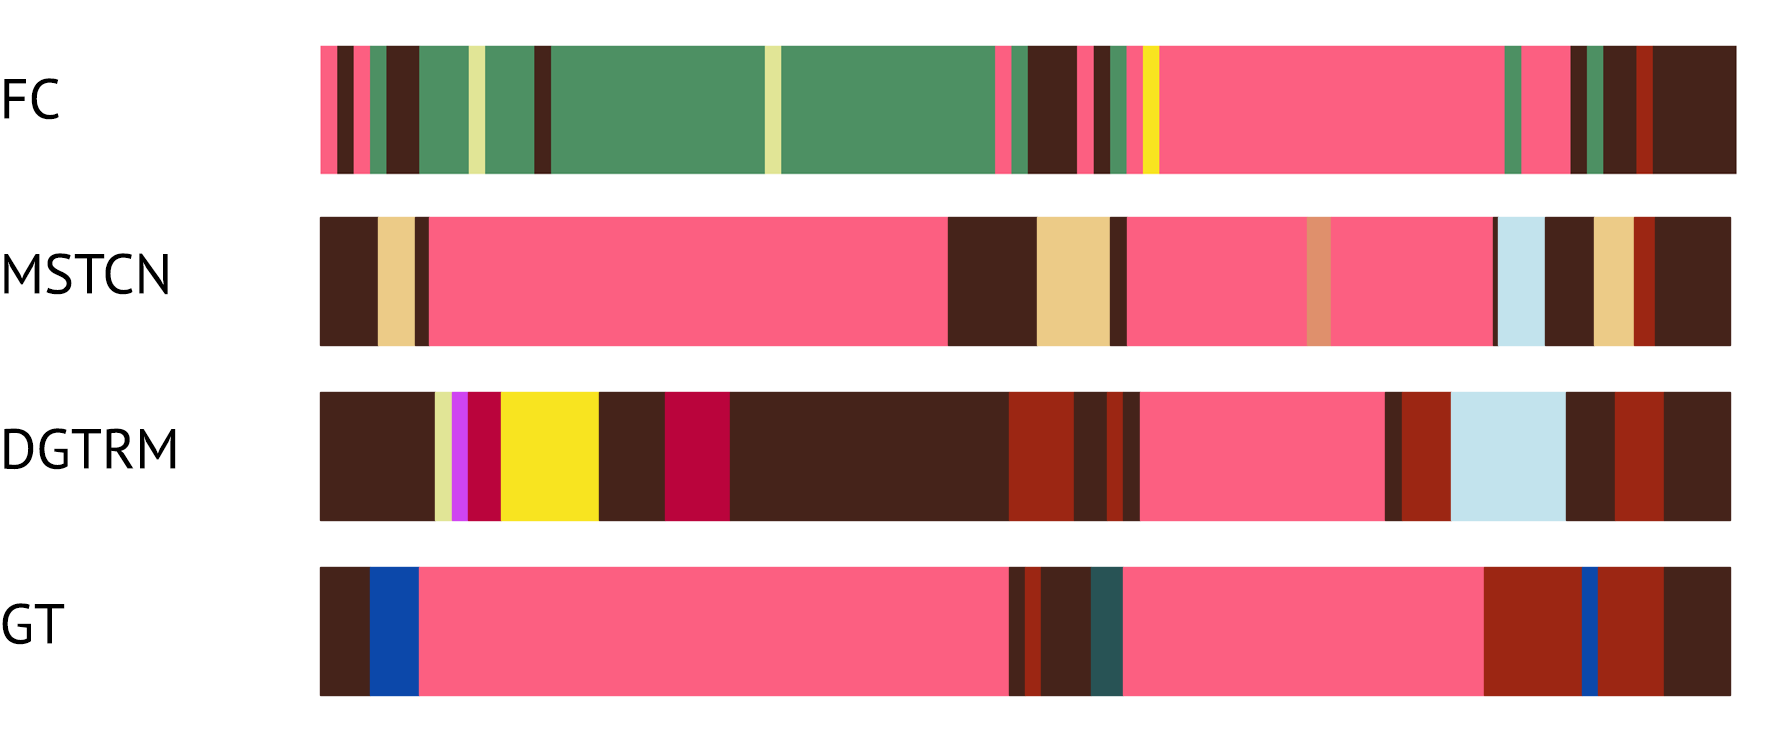
\includegraphics[scale=0.12]{figures/P26_39-comparison.png}
            \caption{P26\_39}
            \label{fig:2639}
        \end{subfigure}\quad
        \begin{subfigure}[b]{0.475\textwidth}
            \centering
            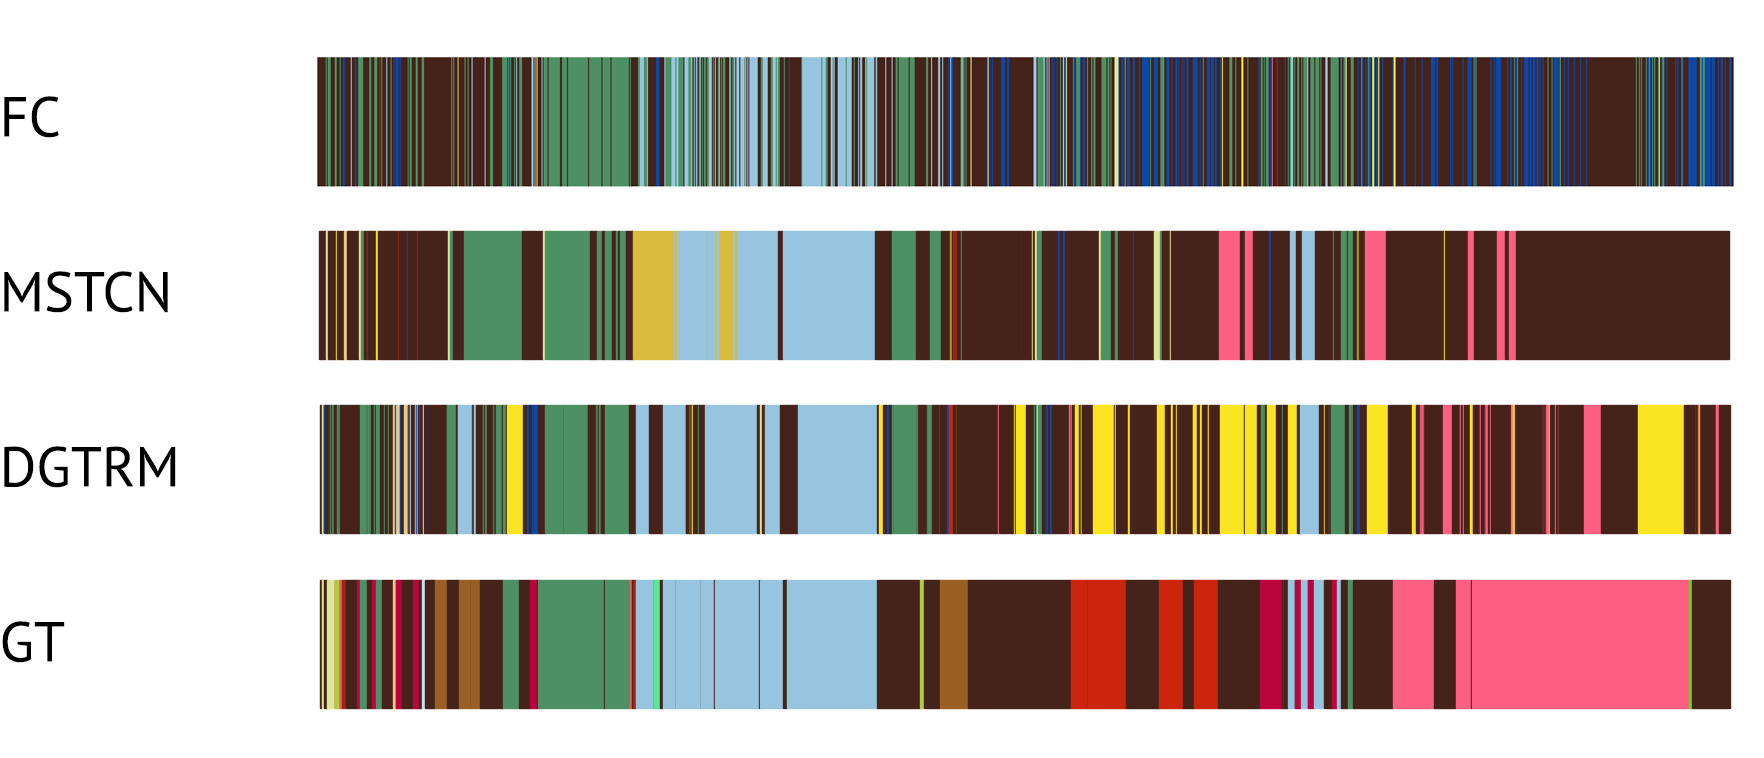
\includegraphics[scale=0.12]{figures/P16_04-comparison.png}
            \caption{P16\_04}
            \label{fig:1604}
        \end{subfigure}
        \caption{Qualitative results of two videos across all models.}
        \label{fig:baseline_qualitative}
    \end{minipage}
\end{center}
\end{figure*}

\paragraph{Metrics} 
We experimented with two variants of loss function: cross-entropy loss with and without weighting. Since background frames comprise a sizable portion, one phenomenon we observe during training is that models tend to classify most of the frames as background, at least in the first few iterations. Down-weighting background classes can mitigate this issue, but inconsistency still exists between the loss function and metrics we used, since classifying frames as the most common verb class (e.g. background, \emph{wash}) can quickly increase frame-wise accuracy until some threshold (usually the percentage of these common verb class). Edit score is a better reflection of the fragmentation issue. Models like MSTCN that incorporate temporal information tend to have higher Edit score than simpler models such as FC.  